\begin{frame}
    \frametitle{Can global methods be applied in Images?}
    \begin{itemize}
        \item Raw pixels do not have semantics
    \end{itemize}
    \begin{figure}
        \centering
        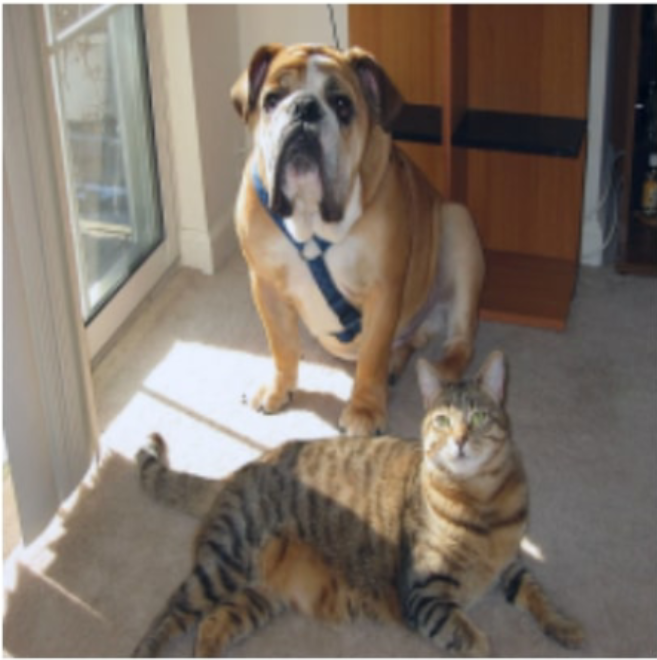
\includegraphics[width=0.49\textwidth]{grad_cam_1}
        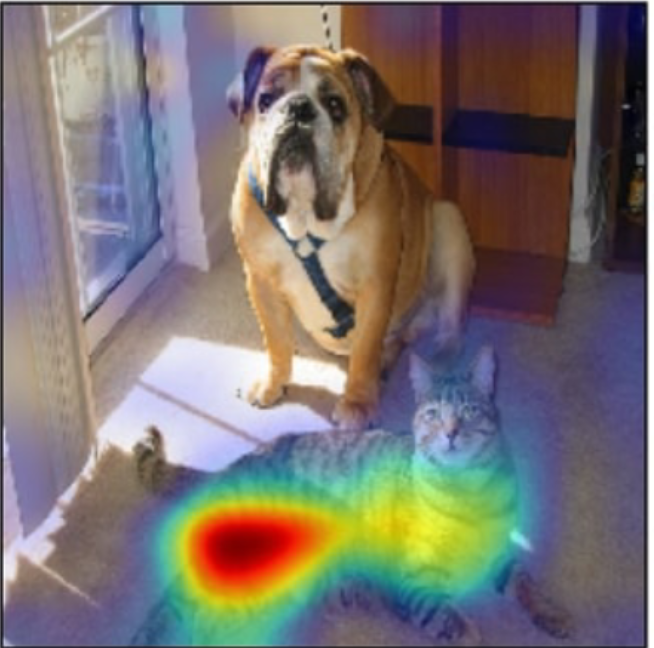
\includegraphics[width=0.49\textwidth]{grad_cam_2}
        \caption{Grad-Cam, image taken from \href{https://arxiv.org/pdf/1610.02391.pdf}{Adebayo et. al (2017)}}
    \end{figure}
\end{frame}


\begin{frame}
    \frametitle{Can global methods be applied in Images?}
    \begin{itemize}
        \item Focus on the reasoning process of the CNN
        \item What makes images (in general) be classified as cats?
        \item Find prototypes!
        \item Unfortunately, not yet available, as a post-hoc explainability technique
        \item Only local prototypes can be found post-hoc
    \end{itemize}

    \begin{figure}
        \centering
        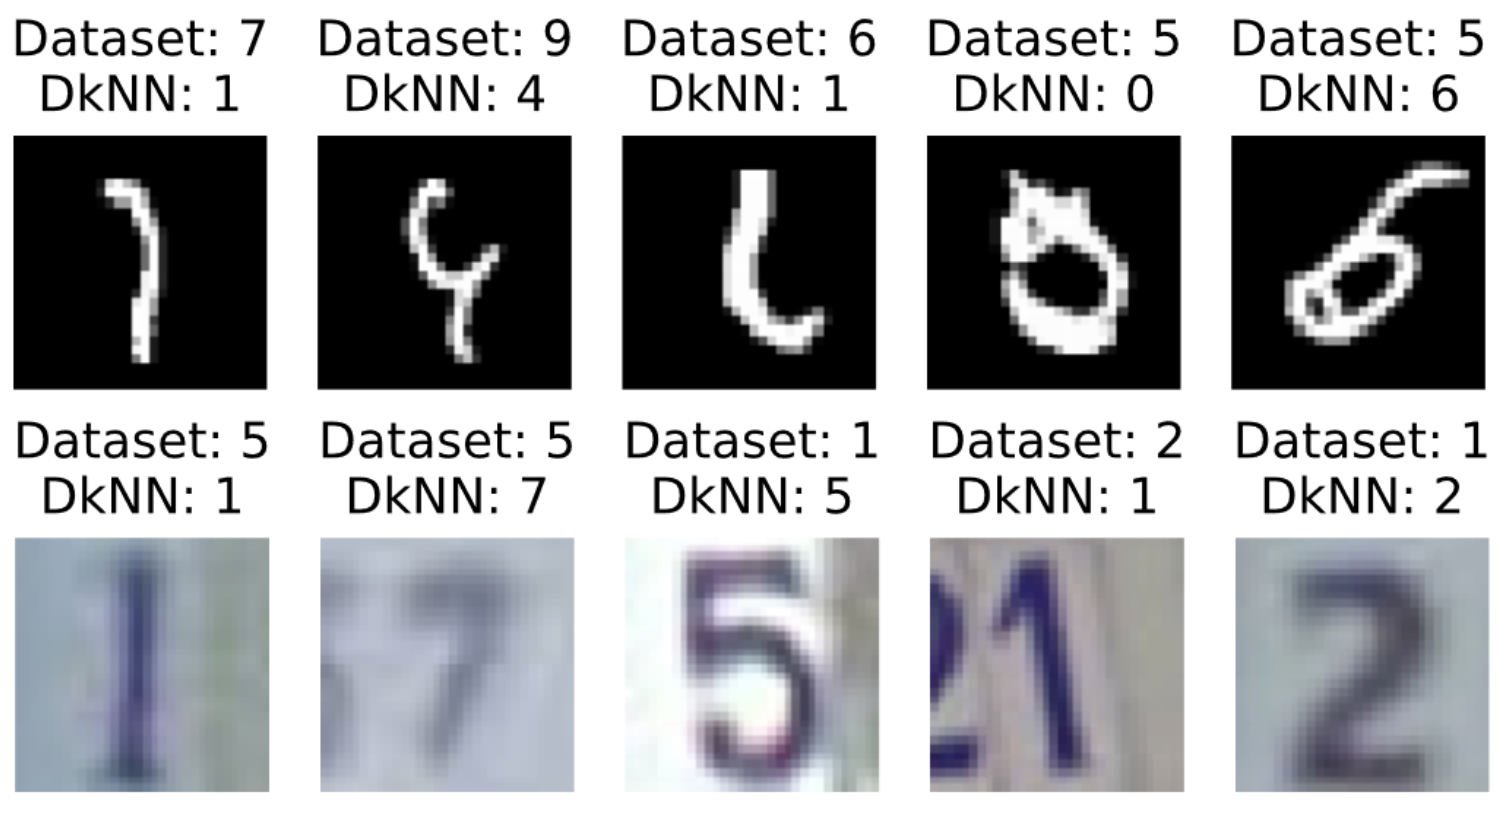
\includegraphics[width=0.49\textwidth]{dknn}
        \caption{Deep KNN, image taken from \href{https://arxiv.org/pdf/1803.04765.pdf}{Papernot et. al (2018)}}
    \end{figure}

\end{frame}


\begin{frame}
    \frametitle{Can global methods be applied in Images?}
    But prototype learning can be enforced in the model architecture
    \begin{figure}
        \centering
        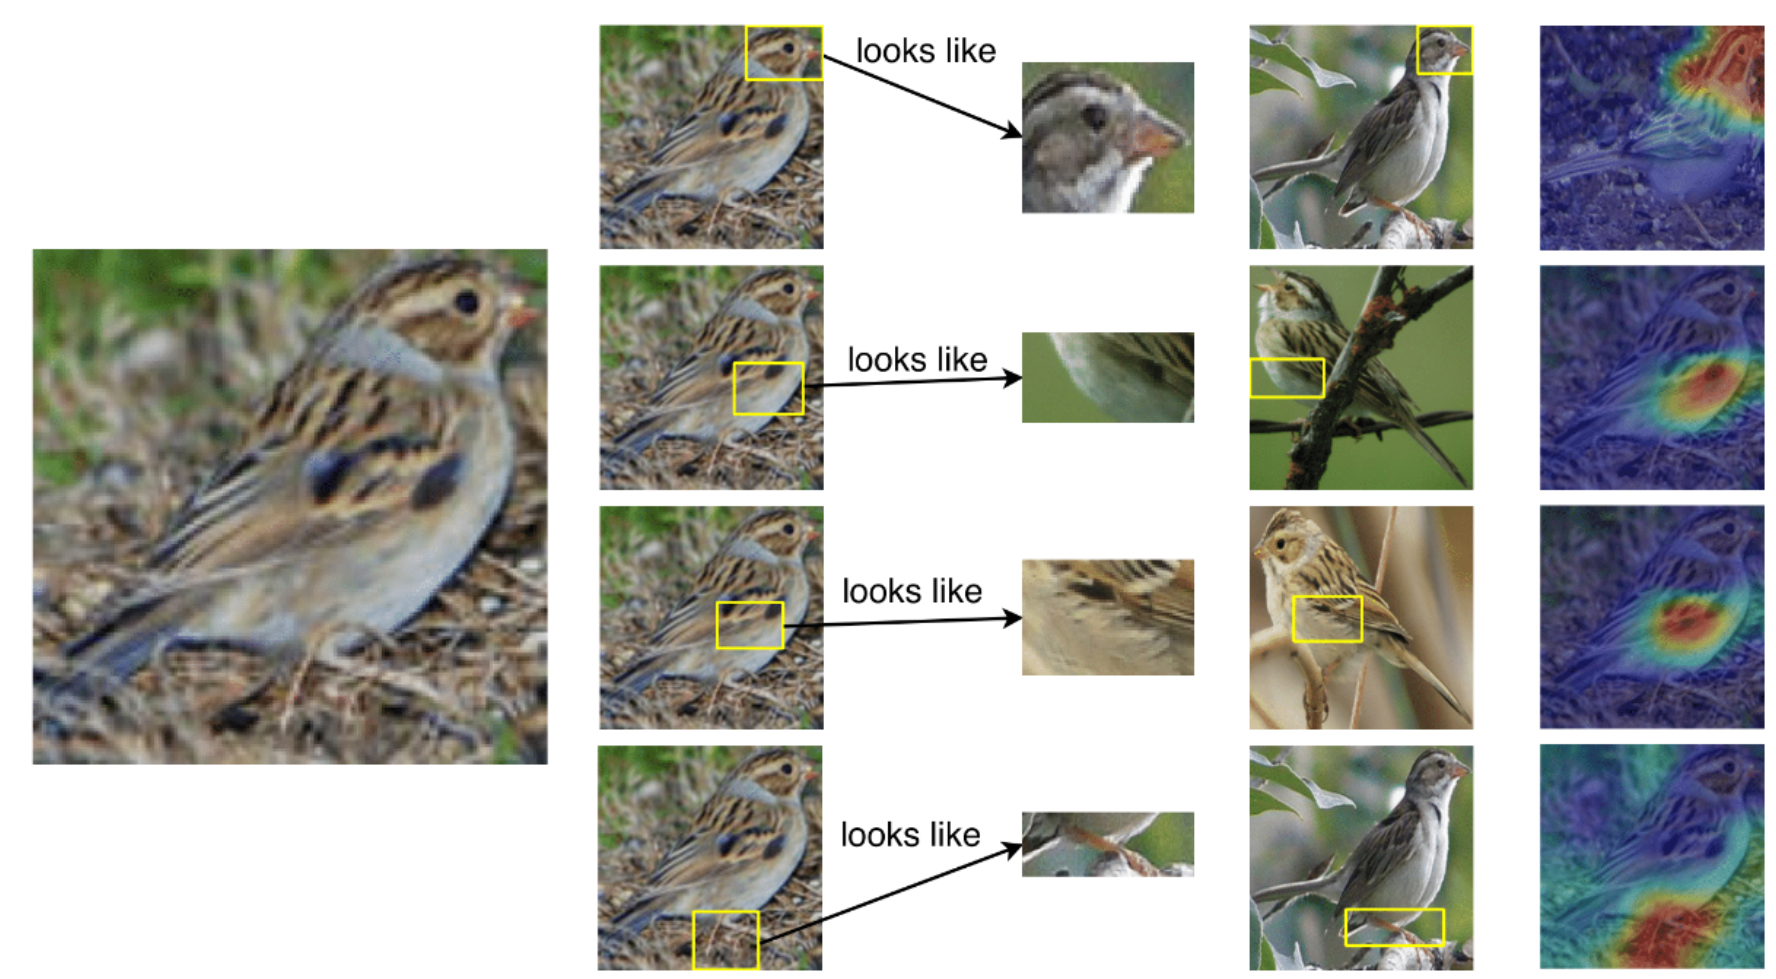
\includegraphics[width=0.7\textwidth]{prototypical_network}
        \caption{Deep KNN, image taken from \href{https://arxiv.org/pdf/1806.10574.pdf}{Chen et. al (2018)}}
    \end{figure}
\end{frame}


